\par
In this chapter, we will discuss about the dataset like how we did the data gathering, what are the steps in data preparation and data pre-processing operations. As I mentioned several times that the success element in a machine learning project doesn't solely depend on the algorithm or model we choose to train the model, but also on the quality of data that is used for the training. These algorithms have a great tendency to learn from whatever dataset it is being fed. Considering this fact, careful steps need to be taken to prevent the model from in-appropriate learning. It has been observed that the biggest challenge during a machine learning project is to clean the dirty data. Roughly, the data scientists spend 60\% of the time in converting the data into a usable form. Most of the time, the dataset we get from the internet or any other source is not accurate, complete and not in ready-to-use state and contains several other things which we do not need. To clean and convert the data into a usable format, there are some fundamental steps that we must follow before using the dataset to train the model like data cleansing which is responsible to remove garbage, irrelevant and redundant data so that we can avoid the false observations. Other than that, there are also several operations we can apply in the pre-processing stage like data augmentation where we transform the data with different metrics like re-scaling, image rotation, zooming, horizontal and vertical flips, etc. The main purpose of data augmentation is to help the model to generalize the data well and avoid overfitting. Furthermore, the dataset we get is normally in raw format and is not in a machine-readable format, so before feeding the data for training, we have to convert the data into a format that can be understood by the machine.
\newline
\par
This thesis aims to develop an intelligent system that can classify the documents automatically. Also, the scope of document classification is very broad as there can be many types of documents. So, considering the time constraints and limits of this thesis, we are focusing on the data which are used for tax claiming purpose. There are several documents that we can use to claim the tax return like income tax statements, salary slips, general purchase receipts, traveling receipts, disability certificates, etc. The above-mentioned documents are somewhat personal and very confidential.
\newline
\par
So, when it comes to the data-gathering phase, the first thing we do is to look up for the dataset from the internet and open-source dataset portals. There are some open-source portals like ImageNet \cite{imgnet} which is an open-source image database, Kaggle Datasets \cite{kaggle_dataset} which is also a database where we can find the data in other formats as well like image, tabular, excel, csv, json, etc. , MNIST \cite{mnist} which is database of hand writing digits, etc where we can find and download different types of data for our machine learning project. However, these databases contain general data like Vehicles dataset, human faces, cats or dogs but the nature of data that we are dealing with in this thesis is quite confidential and is not publicly available in these databases. So, that was the real challenge we faced during this project that we are unable to find any dataset which contains the tax-related documents. Also, the existing automatic document classification projects are mostly for general documents.
\section{Data Gathering}
\par
As I mentioned above that we have narrowed down the scope of documents to tax-related documents and in this thesis, the documents that we are specifically classifying are Income Tax Statement (Lohnsteuerbeschinigung), Salary slips (Gehaltabrechnung) and General Receipts (Rechunung). The reason to lower down the document types for classification is the lack of data. Furthermore, this classification is meant to recognize the above documents only in German language. Since these documents are not available in open-source databases, so we have gathered the data by random google search or collecting the data from colleagues. Some of the data was provided by the company as well. Here, I would like to highlight a fact that the problem with these three document types is that there is not fixed format of these documents and can exist in multiple templates/formats.
\subsection{Income Tax Statement}
If we talk about the income tax statement formats in Germany, then it also has a bit different formats for different years but overall we can say that it shares a partially same format in each template. We researched the formats for the past 15 years and come up with 4 different formats. All these documents are downloaded from the website of the Federal Ministry of Finance \q{www.bundesfinanzministerium.de}. As we can see, the right part of tabular data is the same for each format however the left part for the personal information is changing and occurring in different positions. Please see the below Figure \ref{ls_formats} to check one of the formats that we are using for the classification of the income tax statement. 
\begin{figure}[H]
\centering
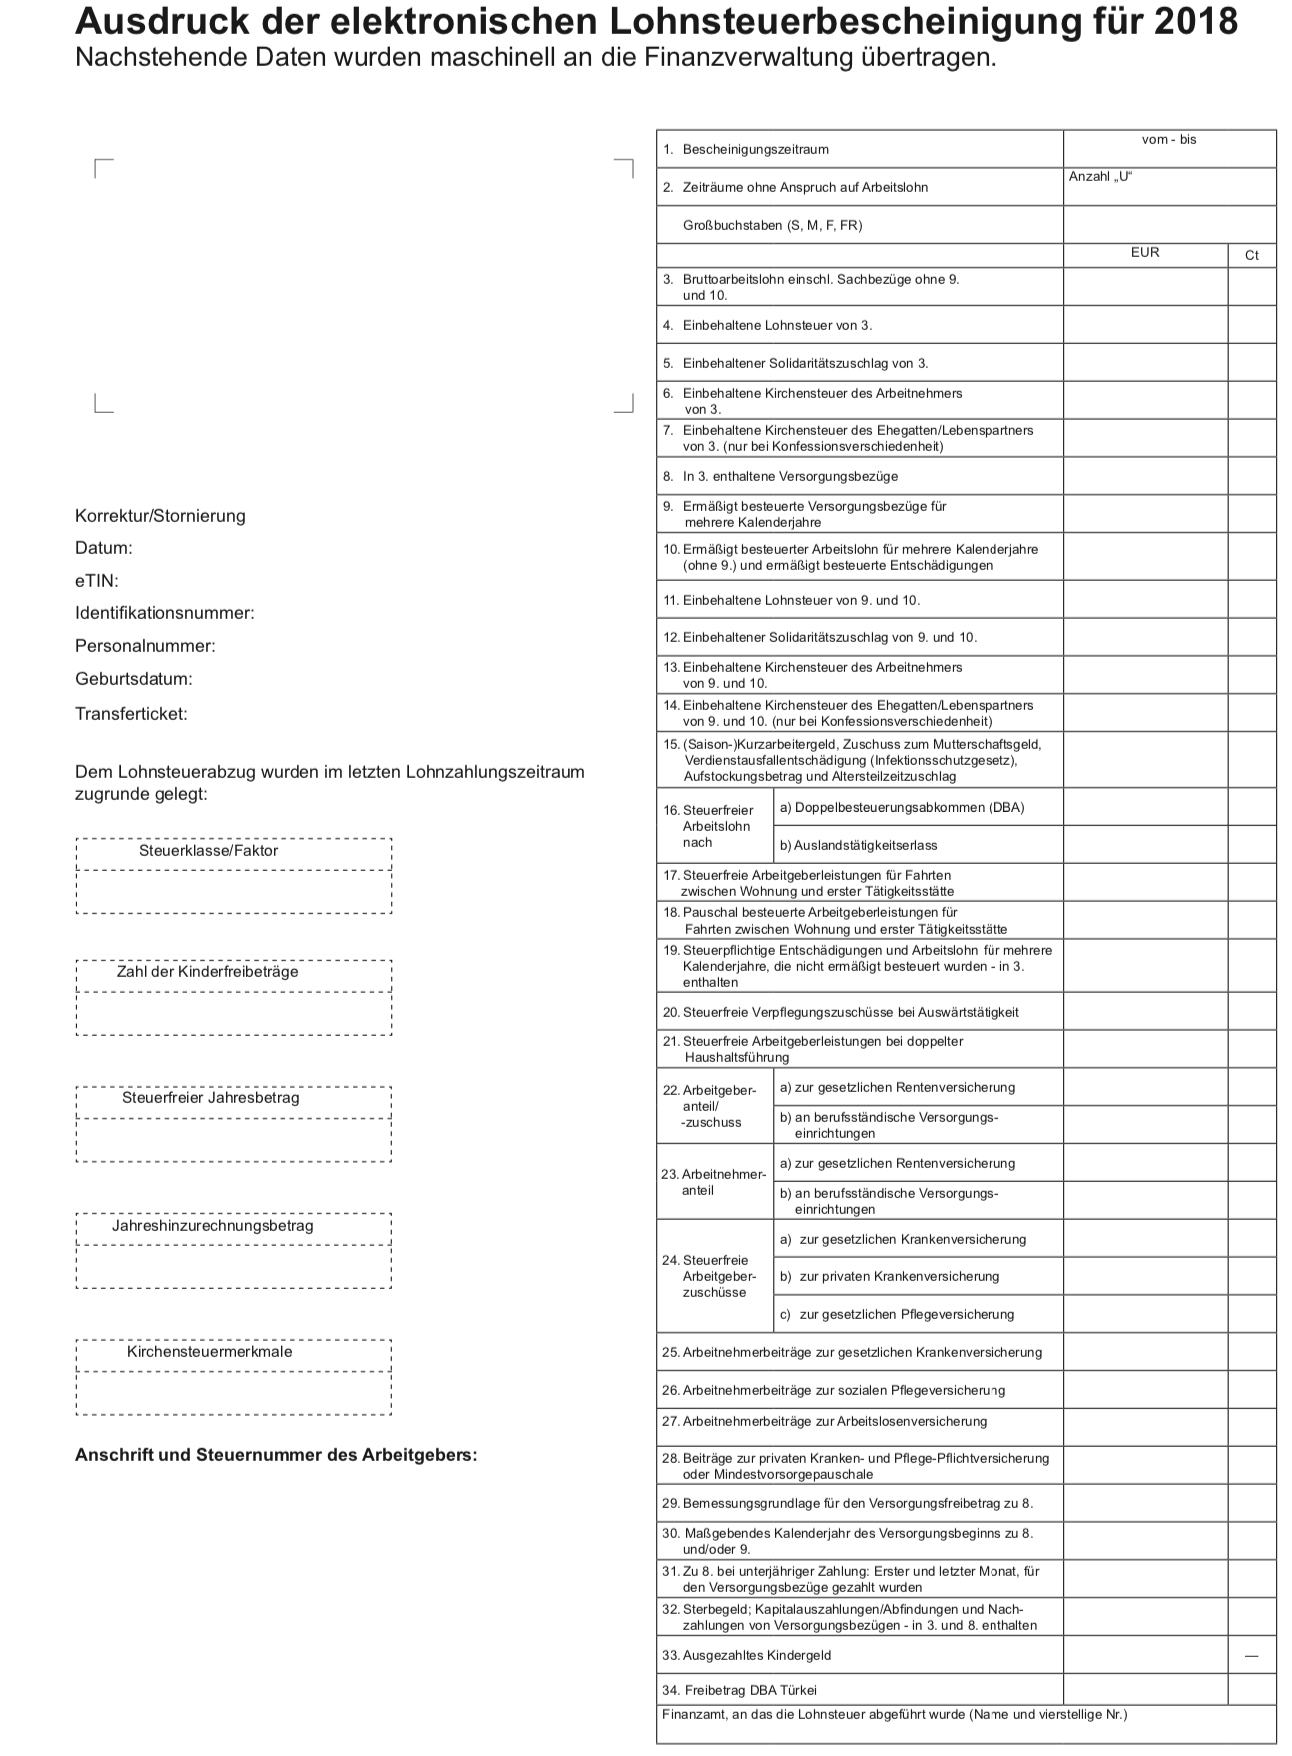
\includegraphics[scale=0.6]{images/Chapter3/ls-format-1.png}
\caption{Income Tax Statement format for classification}
\label{ls_formats}
\end{figure}
\par
\subsection{Salary Slips}
The case of salary slip documents is different from income tax statements because first of all it is not much available on any public site and secondly there can be various formats for this type. For example, if we see different organizations then each one has its own format of salary slip, therefore, we can't really rely on a single format and need to gather the different formats as much as possible. For this thesis, we gathered 4 different formats of this document type from the internet. Please see the below Figure \ref{ga_formats} to check one of the formats that we are using for the classification of salary slips.
\begin{figure}[H]
\centering
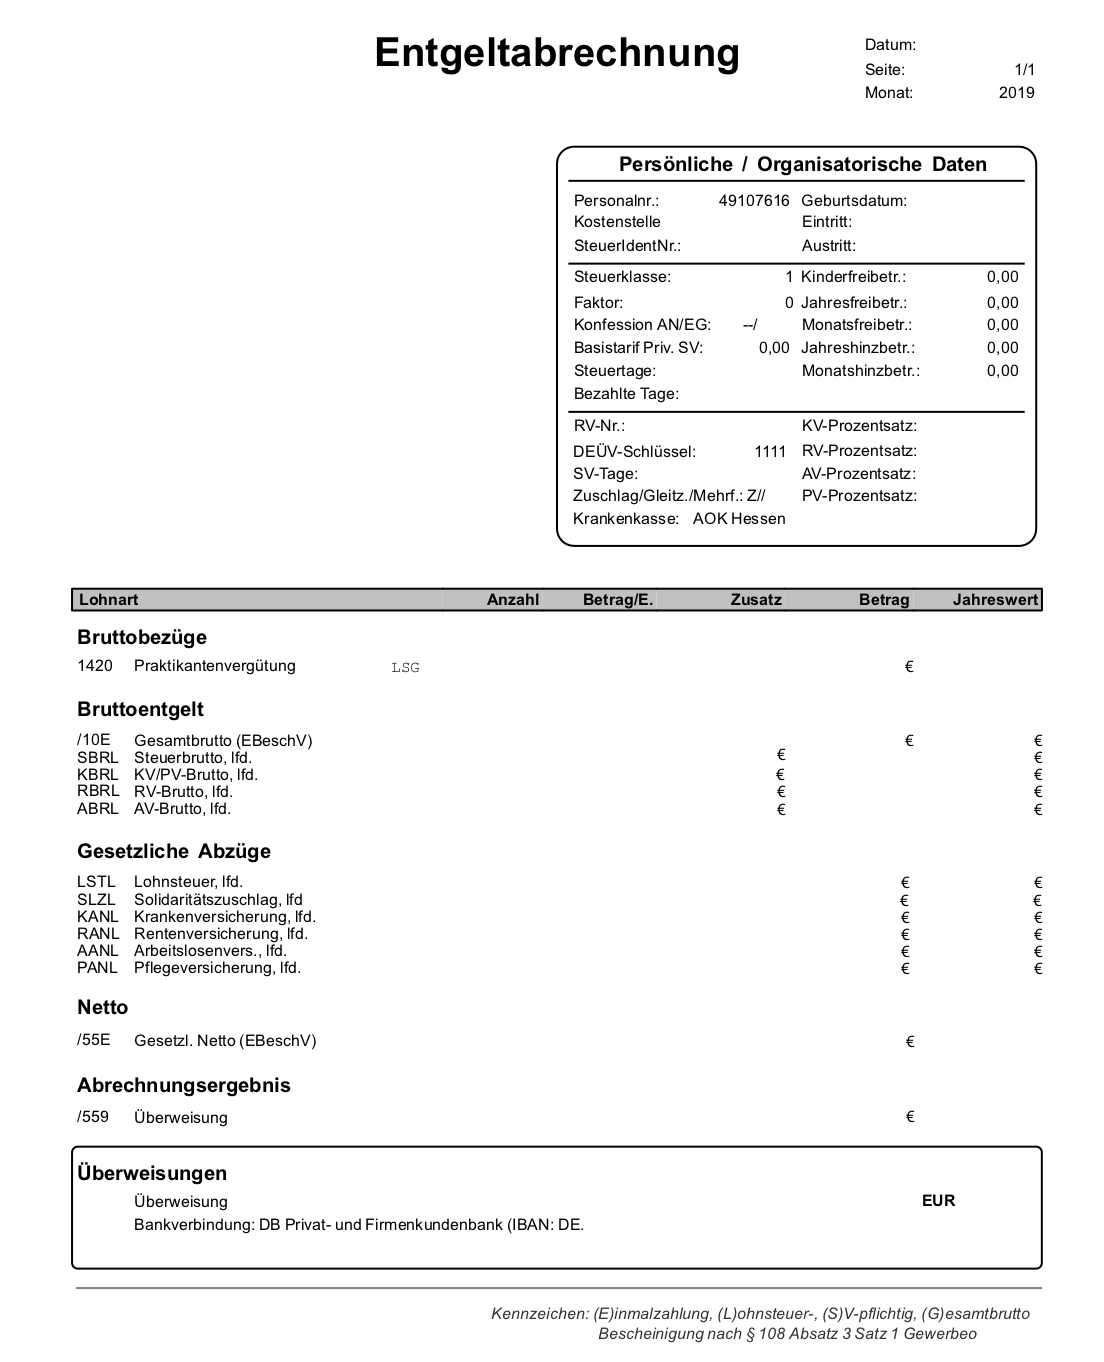
\includegraphics[scale=0.8]{images/Chapter3/ga-format-1.png}
\caption{Salary slip format for classification}
\label{ga_formats}
\end{figure}
\par
\subsection{General Receipts}
It is also the same in the case of general receipts. It is also not much publicly available and can occur in various formats. For this classification, receipts can be of different types like car rental receipts, traveling tickets of the airplane, railway or taxi, purchase receipts for educational purposes if the person is student, etc. We can use these slips to claim the tax. But as compared to the other two documents it is not that much confidential. For this document, we collected the data from our company colleagues and also some from the internet and are using 7 different formats. Please see the below Figure \ref{gr_formats} to check one of the formats that we are using for the classification of general receipts. 
\begin{figure}[H]
\centering
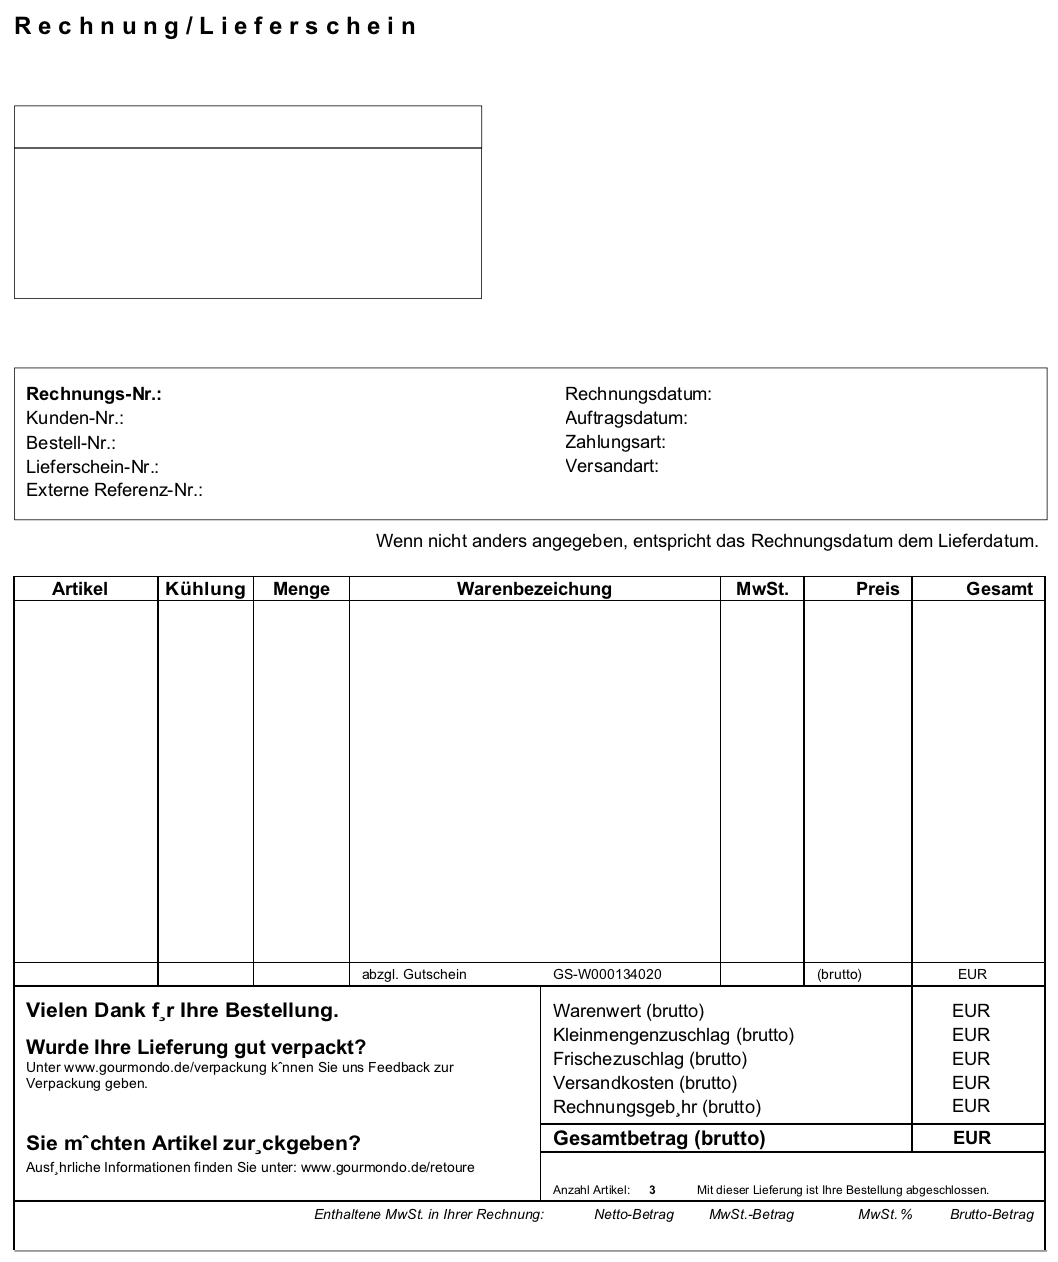
\includegraphics[scale=0.6]{images/Chapter3/gs-format-1.png}
\caption{General Receipts format for classification}
\label{gr_formats}
\end{figure}
\section{Dataset Generation \& Preparation}
So far, we have collected different formats for each document types and now we have to generate the data by using the collected formats. For this purpose, we created a separate project based on node.js which is used for data generation. We have different formats for each document type and based on these formats we generated further data. These formats that we collected are in pdf format. Now, the next thing is to generate or print more pdfs for each document type. Here, we took the help of existing node.js packages and used \q{HummusRecipe} \cite{hummus_recipe} which is a node.js library to create pdfs or to modify an existing pdf. Our task was to take a pdf format of document types as an input, modify that pdf and print the values and save it as a new pdf. So, we took this approach to generate several pdf for each document type. This process was very hectic because, to print any value in the pdf, we have to define the coordinates of the position where we want to print the values. Since there were many values in every document type and this task was hit and trial process to find the right position for any value so it took a lot of time to generate the pdfs. These pdfs were used as training data for two text-based solutions that we provided. In our third and main solution, we are using images as training data to train our model. So, to generate images we again took the help of another node.js package called \q{pdf-poppler} \cite{pdf_poppler}. It is a node.js library which is used to convert pdf files into images and is very fast in terms of performance. So, after generating the pdfs, we generated the images for all the pdfs of different document types. Now, we the training data in two different formats which are pdfs and images which we are using in different solutions.
\begin{table}[H]
\centering
\begin{tabular}{l | l }
Document Types & No. of dataset\\
\hline
Income Tax Statement & 4000 \\
Salary slips & 4000 \\
General Receipts & 4000
\end{tabular}
\caption{Overview of number of dataset generated for three different types of tax-related document}
\label{dataset_count}
\end{table}
\subsection{Dataset preparation for Solution I}
In this solution, we are using our generated dataset in the form of pdfs. Since this is a non-machine learning solution so there is no need for a high amount of data because there is no training involved. This solution is based on textual data, so we look for the meaningful keywords and categorize it according to the document types and assign weights by its frequency. During the prediction, we tokenize the input text and check the score of each document type and returns the type with higher frequency. To generate the dictionary of words with weights, we are using the dataset in the following quantity.
\begin{table}[H]
\centering
\begin{tabular}{l | l }
Document Types & No. of dataset\\
\hline
Income Tax Statement & 200 \\
Salary slips & 200 \\
General Receipts & 200
\end{tabular}
\caption{Overview of number of dataset using to generate Word dictionary}
\label{dataset_count_sol1}
\end{table}
\subsection{Dataset preparation for Solution II}
For Solution II, we are using our generated dataset in the form of pdfs as well. This solution is based on machine learning techniques and is using textual data as input for training. To generate a dataset for training, we are extracting the data from all the pdfs and storing it in an array. Here, I would like to mention that since the string that is extracted from the pdf is most of the time same for a document type and is very long too. For example, in the income tax statement, the text from each document is same and due to which if we directly use this data then each training record for income statement will be the same. To avoid this situation and to introduce some variation, we broke the string into multiple small string and at the same time shuffled it as well so that data record does not have similar content. After breaking the string, the array will become larger too with somewhat different content at each index. Following are the number of pdfs we are using to generate the dataset. 
\begin{table}[H]
\centering
\begin{tabular}{l | l }
Document Types & No. of dataset\\
\hline
Income Tax Statement & 4000 \\
Salary slips & 4000 \\
General Receipts & 4000
\end{tabular}
\caption{Overview of number of dataset using to train the model}
\label{dataset_count_sol2}
\end{table}
\par
In total, we are using 4000 datasets for each document type which is in total becomes 12000 documents and split ratio for test and train is 80\% and 20\% respectively. Please refer to the below Table \ref{record_count_sol2} for the numbers for the test and train split ratio. Here, I would like to mention that these numbers are the number of records in the array after breaking the extracted string from pdfs into further small strings that is why the figures are bigger than the number of documents.
\begin{table}[H]
\centering
\begin{tabular}{l | l }
Split Type & No. of records\\
\hline
Train & 18924 \\
Test & 4731
\end{tabular}
\caption{Overview of number of records using to train the model by split type}
\label{record_count_sol2}
\end{table}
\subsection{Dataset preparation for Solution III}
In the third solution, we are using our generated dataset in the form of images. This solution is also based on machine learning techniques but here we are using image data as input to train our model. Considering the size of the dataset, we didn't break our dataset in chunks and trained the model at once. Following are the number of images we are using to train the model. 
\begin{table}[H]
\centering
\begin{tabular}{l | l }
Document Types & No. of dataset\\
\hline
Income Tax Statement & 4000 \\
Salary slips & 4000 \\
General Receipts & 4200
\end{tabular}
\caption{Overview of number of dataset using to train the model}
\label{dataset_count_sol3}
\end{table}
\par
In this solution, we are using 4000 images for income tax statements and salary slips and 4200 images for general receipts which in total becomes 12200 images. The split ratio for train, test and validation set is 60\%, 25\%, and 15\% respectively. Following are the tables for the exact amount of dataset for train, test, and validation
\begin{table}[H]
\centering
\begin{tabular}{l | l }
Document Types & No. of dataset (Train Split)\\
\hline
Income Tax Statement & 2377 \\
Salary slips & 2354 \\
General Receipts & 2528
\end{tabular}
\caption{Overview of number of dataset using to train the model for train split}
\label{dataset_count_sol3_training}
\end{table}
\begin{table}[H]
\centering
\begin{tabular}{l | l }
Document Types & No. of dataset (Test Split)\\
\hline
Income Tax Statement & 616 \\
Salary slips & 608 \\
General Receipts & 606
\end{tabular}
\caption{Overview of number of dataset using to train the model for test split}
\label{dataset_count_sol3_test}
\end{table}
\begin{table}[H]
\centering
\begin{tabular}{l | l }
Document Types & No. of dataset (Validation Split)\\
\hline
Income Tax Statement & 1007 \\
Salary slips & 1038 \\
General Receipts & 1066
\end{tabular}
\caption{Overview of number of dataset using to train the model for validation split}
\label{dataset_count_sol3_validation}
\end{table}
\section{Data Pre-processing \& Augmentation}
Data pre-processing is a stage where we apply several techniques to the dataset to make it well understandable to the model. It is very important to spend some time in data pre-processing because from this stage we will feed the data to our model and we have to make sure that our model should generalize the data well. Furthermore, we also apply the augmentation technique on the dataset where we transform our data into different shapes with the help of certain augmentation metrics and parameters.
\newline
\par
In the pre-processing step, we also have to make sure that the image should contain only one image. Since we generated the image by converting the pdfs into images. There were some templates which comprise of two pages, so at that time, we avoid those templates and made sure to choose the right templates. After getting the images, in this step, we also resized the image into 224 x 224. The purpose of this resizing is the requirement of the transfer learning model VGG19 that we are using to train the model as it accepts only the images with the height and width of 224.
\subsection{Data Augmentation}
We have discussed earlier that the kind of dataset we are dealing with does not have much variation and also, for now, we have limited formats for each document type. To obtain a well-trained model, we have to feed the data to the model with different variations. One way to overcome this problem to do data(image) augmentation. Image augmentation is a method by which we generate more data by applying several augmentation parameters. For the image augmentation, we are using the Keras library \cite{keras} which has a class called ImageDataGenerator \cite{keras_ip} that provides the image augmentation service. Please find below the Figure to find out the parameters we are using for image augmentation.
\begin{figure}[H]
\centering
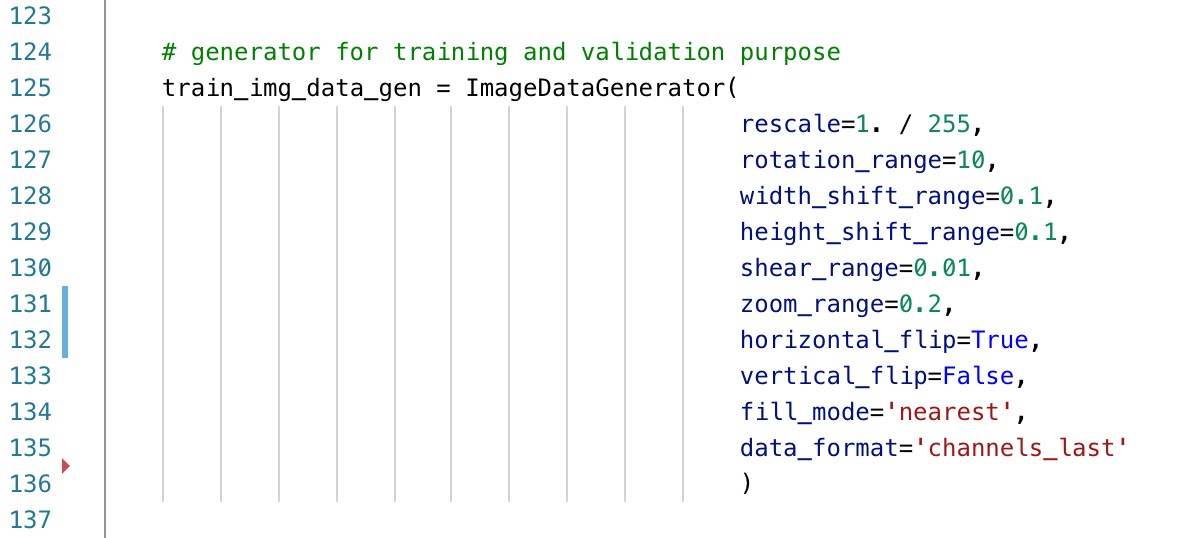
\includegraphics[scale=0.6]{images/Chapter3/augmentation_metrics.png}
\caption{Parameters for Image Augmentation}
\label{ia_params}
\end{figure}
\par
Here, we will explain the parameters a little. As we can see we are applying several parameters to transform the image like rescale which is used to reduce the pixel size of the image to overcome the computing time overhead by dividing each pixel by 255. We are also rotating images as well. It is very important to have some data with a bit rotated form because it is quite common that when it will be used in real-world for classification then most of the people just took the photo of document from their mobile and upload the image to the system for classification so we cannot expect the well-positioned or aligned images from user. Width shift range and Height shift range are used to move the image horizontally and vertically respectively. The shear range for randomly applying the shearing transformation. We also applied zoom range to zoom the photo and sets the horizontal flips to true to flip the image horizontally sometimes. We disabled the vertical flips because it doesn't make sense in our situation. Please see Figure \ref{aug_data} to see the transformation of images after applying augmentation.
\begin{figure}[H]
\centering
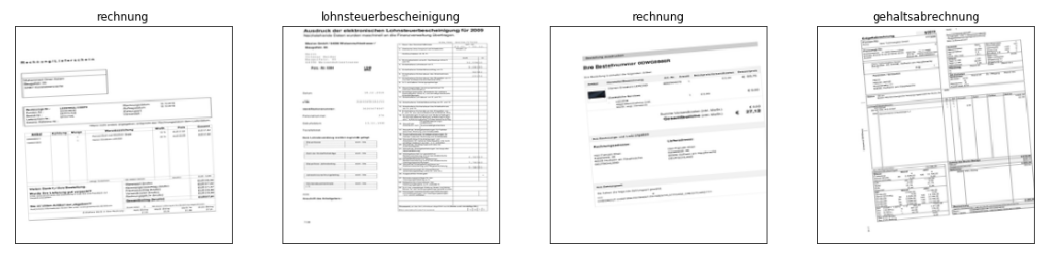
\includegraphics[scale=0.7]{images/Chapter3/augmented_data.png}
\caption{Images after Image Augmentation}
\label{aug_data}
\end{figure}